\documentclass[../psets.tex]{subfiles}

\pagestyle{main}
\renewcommand{\leftmark}{Problem Set \thesection}

\begin{document}




\section{The Kinetic Theory of Gases}
\emph{From \textcite{bib:McQuarrieSimon}.}
\subsection*{Chapter 27}
\begin{enumerate}[label={\textbf{27-\arabic*.}},leftmargin=3.5em]
    \setcounter{enumi}{4}
    \item Arrange the following gases in order of increasing root-mean-square speed at the same temperature: \ce{O2}, \ce{N2}, \ce{H2O}, \ce{CO2}, \ce{NO2}, \ce{{}^235UF6}, \ce{{}^238UF6}.
    \stepcounter{enumi}
    \item The speed of sound in an ideal monatomic gas is given by
    \begin{equation*}
        u_\text{sound} = \sqrt{\frac{5RT}{3M}}
    \end{equation*}
    Derive an equation for the ratio $u_\text{rms}/u_\text{sound}$. Calculate the root-mean-square speed for an argon atom at \SI{20}{\celsius} and compare your answer to the speed of sound in argon.
    \setcounter{enumi}{11}
    \item We can use the equation for $f(u_x)$ to calculate the probability that the $x$-component of the velocity of a molecule lies within some range. For example, show that the probability that $-u_{x0}\leq u_x\leq u_{x0}$ is given by
    \begin{align*}
        \Prob\{-u_{x0}\leq u_x\leq u_{x0}\} &= \sqrt{\frac{m}{2\pi\kB T}}\int_{-u_{x0}}^{u_{x0}}\e[-mu_x^2/2\kB T]\dd{u_x}\\
        &= 2\sqrt{\frac{m}{2\pi\kB T}}\int_0^{u_{x0}}\e[-mu_x^2/2\kB T]\dd{u_x}
    \end{align*}
    Now let $mu_x^2/2\kB T=w^2$ to get the cleaner looking expression
    \begin{equation*}
        \Prob\{-u_{x0}\leq u_x\leq u_{x0}\} = \frac{2}{\sqrt{\pi}}\int_0^{w_0}\e[-w^2]\dd{w}
    \end{equation*}
    where $w_0=u_{x0}\sqrt{m/2\kB T}$.\par
    It so happens that the above integral cannot be evaluated in terms of any function that we have encountered up to now. It is customary to express the integral in terms of a new function called the \textbf{error function}, which is defined by
    \begin{equation*}
        \erf(z) = \frac{2}{\sqrt{\pi}}\int_0^z\e[-x^2]\dd{x}
    \end{equation*}
    The error function can be evaluated as a function of $z$ by evaluating its defining integral numerically. Some values of $\erf(z)$ are
    \begin{center}
        \small
        \renewcommand{\arraystretch}{1.4}
        \begin{tabular}{cc|cc}
            $z$ & $\erf(z)$ & $z$ & $\erf(z)$\\
            \hline
            0.20 & 0.22270 & 1.20 & 0.91031\\
            0.40 & 0.42839 & 1.40 & 0.95229\\
            0.60 & 0.60386 & 1.60 & 0.97635\\
            0.80 & 0.74210 & 1.80 & 0.98909\\
            1.00 & 0.84270 & 2.00 & 0.99532\\
        \end{tabular}
    \end{center}
    Now show that
    \begin{equation*}
        \Prob\{-u_{x0}\leq u_x\leq u_{x0}\} = \erf(w_0)
    \end{equation*}
    Calculate the probability that $-\sqrt{2\kB T/m}\leq u_x\leq\sqrt{2\kB T/m}$.
    \setcounter{enumi}{19}
    \item Show that the variance of the equation $I(\nu)\propto\e[-mc^2(\nu-\nu_0)^2/2\nu_0^2\kB T]$ is given by $\sigma^2=\nu_0^2\kB T/mc^2$. Calculate $\sigma$ for the $3p$ ${}^2P_{3/2}$ to $3s$ ${}^2S_{1/2}$ transition in atomic sodium vapor (see Figure 8.4 on \textcite[307]{bib:McQuarrieSimon}) at \SI{500}{\kelvin}.
    \setcounter{enumi}{23}
    \item Show that the probability that a molecule has a speed less than or equal to $u_0$ is given by
    \begin{equation*}
        \Prob\{u\leq u_0\} = \frac{4}{\sqrt{\pi}}\int_0^{x_0}x^2\e[-x^2]\dd{x}
    \end{equation*}
    where $x_0=u_0\sqrt{m/2\kB T}$. This integral cannot be expressed in terms of any known function and must be integrated numerically. Use Simpson's rule or any other integration routine to evaluate $\Prob\{u\leq\sqrt{2\kB T/m}\}$.
    \setcounter{enumi}{26}
    \item Derive an expression for $\sigma_\varepsilon^2=\prb{\varepsilon^2}-\prb{\varepsilon}^2$ from the equation for $F(\varepsilon)\dd{\varepsilon}$. Now form the ratio $\sigma_\varepsilon/\prb{\varepsilon}$. What does this say about the fluctuation in $\varepsilon$?
    \setcounter{enumi}{33}
    \item The figure below illustrates another method that has been used to determine the distribution of molecular speeds.
    \begin{figure}[H]
        \centering
        \footnotesize
        \begin{subfigure}[b]{0.49\linewidth}
            \centering
            \begin{tikzpicture}[
                every path/.style={semithick}
            ]
                \path (-4,0) -- (4,0);
    
                \draw circle (2cm);
                \draw [double=white,double distance=1mm] (-2.1,0) -- (-1.9,0);
                \draw [white,line width=1mm] (-2.2,0) -- (-1.8,0);
    
                \draw [-latex] (0,0) -- node[below right=-2pt]{$R$} (45:2);
                \draw [-latex] (-2.5,0) node[left,align=center]{Pulse of\\molecules} -- (-1.5,0);
                \draw [decorate,decoration={text along path,text=Direction of drum rotation}] (120:2.2) arc[start angle=120,end angle=-90,radius=2.2cm];
                \draw [-latex] (123:2.28) arc[start angle=123,end angle=150,radius=2.28cm];
            \end{tikzpicture}
            \caption{}
        \end{subfigure}
        \begin{subfigure}[b]{0.3\linewidth}
            \centering
            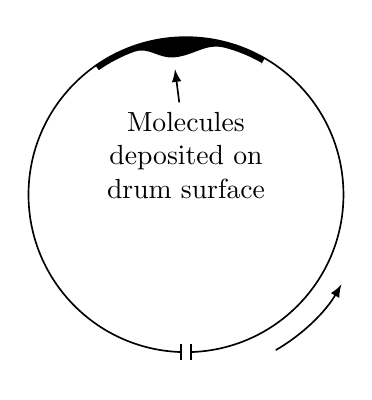
\begin{tikzpicture}[
                every path/.style={semithick}
            ]
                \draw circle (2cm);
                \draw [double=white,double distance=1mm] (-90:2.1) -- (-90:1.9);
                \draw [white,line width=1mm] (-90:2.2) -- (-90:1.8);
    
                \fill (60:1.9)
                    -- (60:2)
                    arc[start angle=60,end angle=125,radius=2cm]
                    -- (125:1.93)
                    arc[start angle=125,end angle=110,radius=1.93cm]
                    to[out=20,in=-175] (95:1.75)
                    to[out=5,in=165] (75:1.93)
                    arc[start angle=75,end angle=60,radius=1.93cm]
                    -- cycle
                ;
                \node [align=center] at (0,0.5) {Molecules\\deposited on\\drum surface}
                    edge [-latex] (95:1.6);
                ;
    
                \draw [-latex] (-60:2.28) arc[start angle=-60,end angle=-30,radius=2.28cm];
            \end{tikzpicture}
            \caption{}
        \end{subfigure}
    \end{figure}
    A pulse of molecules collimated from a hot oven enters a rotating hollow drum. Let $R$ be the radius of the drum, $\nu$ be the rotational frequency, and $s$ be the distance through which the drum rotates during the time it takes for a molecule to travel from the entrance slit to the inner surface of the drum. Show that
    \begin{equation*}
        s = \frac{4\pi R^2\nu}{u}
    \end{equation*}
    where $u$ is the speed of the molecule.\par
    Use the equation for $\dd{z_\text{coll}}$ to show that the distribution of molecular speeds emerging from the over is proportional to $u^3\e[-mu^2/2\kB T]\dd{u}$. Now show that the distribution of molecules striking the inner surface of the cylinder is given by
    \begin{equation*}
        I(s)\dd{s} = \frac{A}{s^5}\e[-m(4\pi R^2\nu)^2/2\kB Ts^2]\dd{s}
    \end{equation*}
    where $A$ is simply a proportionality constant. Plot $I$ versus $s$ for various values of $4\pi R^2\nu/\sqrt{2\kB T/m}$, say 0.1, 1, and 3. Experimental data are quantitatively described by the above equation.
    \setcounter{enumi}{35}
    \item On the average, what is the time between collisions of a xenon atom at \SI{300}{\kelvin} and\dots
    \begin{enumerate}
        \item One torr;
        \item One bar.
    \end{enumerate}
    \setcounter{enumi}{39}
    \item The following table gives the pressure and temperature of the Earth's upper atmosphere as a function of altitude.
    \begin{center}
        \small
        \renewcommand{\arraystretch}{1.2}
        \begin{tabular}{ccc}
            Altitude (\si{\kilo\meter}) & Pressure (\si{\milli\bar}) & Temperature (\si{\kelvin})\\
            \hline
            20.0 & 56 & 220\\
            40.0 & 3.2 & 260\\
            60.0 & 0.28 & 260\\
            80.0 & 0.013 & 180\\
        \end{tabular}
    \end{center}
    Assuming for simplicity that air consists entirely of nitrogen, calculate the mean free path at each of these conditions.
\end{enumerate}




\end{document}